\documentclass[12pt]{article}

\usepackage{amsmath}
\usepackage{graphicx}

\title{A response to the review of the manuscript
``Seeq: a library for inexact DNA sequence matching''}
\date{}

\newenvironment{code}{\ttfamily}{\par}

\begin{document}
\maketitle
As the authors of the manuscript ``Seeq: a library for inexact
DNA sequence matching'', we would like to discuss some of the
ideas that were raised by the reviewers. We believe that
critical discussion, based on facts and arguments is fundamental
to the scientific process. We fully respect the decision of the
editor and of our peers, but we do not consider that we should
interrupt a fertile discussion because the manuscript was
rejected. Please do not see in this letter a criticism of the
reviews, but simply a wish to respond to some of the points that
were raised.

Because this is not a rebuttal, we will do our best to make it
informal and didactic.
But before doing so, we would like to congratulate the reviewers for
a really outstanding work. We are all for software quality and
excellent science, we wish that every tool were scrutinized with
the same amout of care. We have also learned important lessons,
and the suggestions will greatly help us improve the software and
the manuscript.

\section{The inception}

It started from casual Internet
browsing of pages that have little to do with bioinformatics.
The first is a seminal series of blog posts by Cox Russel [1]
explaining how and why he implemented the regular expression library
RE2. The key insight was that many modern regular expression engines
(including those of Perl and Python) have ``forgotten'' the
theory and are clearly dominated by lazy DFA-based implementations.

The second source of inspiration was a blog post by Nick Johnson [2]
where he explains the use of Levenshtein automata in the problem of
approximate string query. In Fig.~\ref{generalities} we give some
generalities about Levenshtein automata, in case the reader is not
familiar with these concepts.

\begin{figure}[!tpb]
\centerline{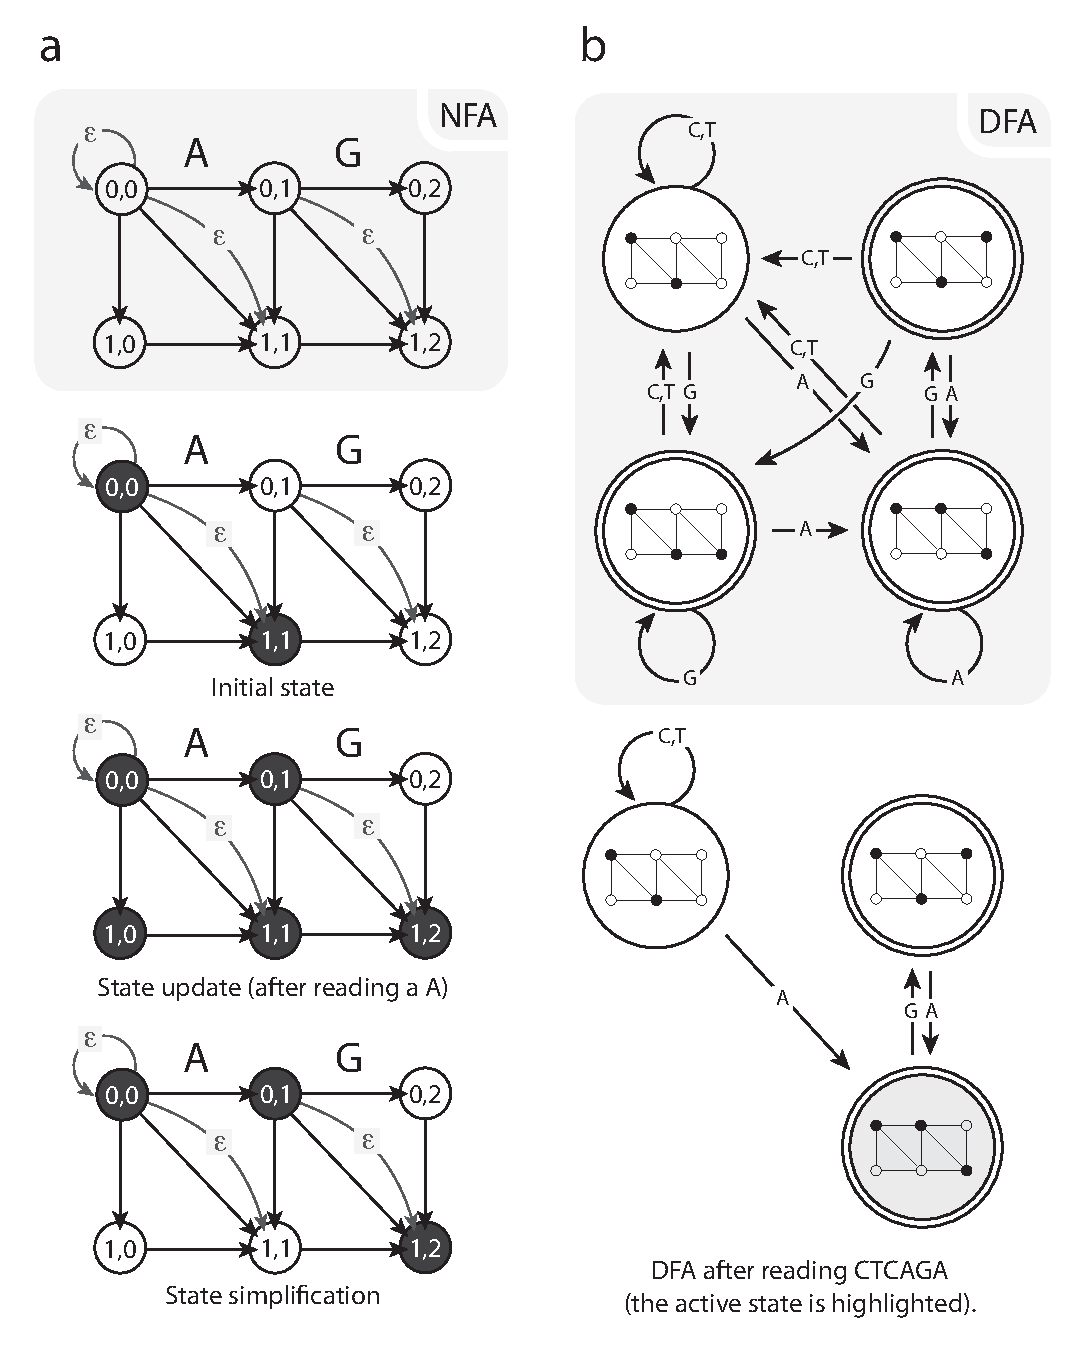
\includegraphics[scale=.6]{edit_matrix.pdf}}
\caption{Generalities on Levenshtein automata. a) Edit graph
of the string \texttt{GA} with 1 tolerated error. The edit graph
is a NFA with state transition as shown in the top panel. States
are labelled by two numbers indicating their number of errors and
their position relative to the search pattern. NFAs can be ins
several active states (dark circles). The initial active states
of the NFA are as shown in the second panel. After reading
\texttt{A} from the input, the active states are updated as shown
on the third panel. The active states can be simplified by keeping
only the upper node on each column, as shown on the bottom panel.
b) DFA representation. Every NFA has a DFAs representation.
States of the DFA are sets of active states of the NFA. In a
lazy DFA, only the states required to process the input are present
(bottom panel).
}\label{generalities}
\end{figure}

When we had to identify spike oligos in our
sequencing experiments, we used the Python implementation suggested
by Nick Johnson, which solved the problem (Illumina sequencing is
not indel-prone, but oligos synthesis is, which is why we needed
the Levenshtein distance). However, the Python prototype was rather
slow, and because it is a non lazy DFA, the memory footprint was high.

We connected the ideas of the two posts, and the first C
implementation of Seeq gave astonishing results. We knew that this
was not novel (lazy DFAs were implemented in egrep since 1989), but
because Seeq was much faster then Myers' bitfield algorithm,
we thought that lazy Levenshtein automata did not quite
make the jump from string processing to bioinformatics and that
someone should tell the community that they are efficient.

\section{Sparsity of the DFA}
\label{sketch}

At that stage, we were both surprised and skeptical. One concern (also
pointed out by reviewer 2) was that the potential number of states
was very high. Our initial implementation was based on the NFA
called the edit graph (Fig.~\ref{generalities}a),
which can be in $2^{(k+1)L}$ states, where $k$
is the tolerated number of errors and $L$ is the length of the
pattern. This number is enormous, but surprisingly, the memory
footprint was never an issue,
even for large files and long patterns. For some reason,
the lazy Levenshtein automaton explored only a small portion of its
states.

We realized that we could reduce the possible number of states by
keeping only the upper envelope of the NFA states in the edit graph
(in the manuscript, we presented states as columns from the alignment
because we thought that bioinformaticians would be more comfortable
with this representation, but the representations are strictly
equivalent). This made Seeq faster and reduced the memory footprint.
And it also allows us to explain why the DFA is sparse.

With this representation, a state is a line of the edit graph that
extends from the top-left
corner. On this line, local maxima have travelled from the top-left
corner by going either to the right (in case of a match) or in
diagonal (in case of a mismatch). So the probability that a local
maximum is at position $(i,j)$, where $(0,0)$ is
the top-left corner is approximately

\begin{equation}
{j \choose i} \left(\frac{3}{4}\right)^i
  \left(\frac{1}{4}\right)^{j-i}.
\end{equation}

This expresses that the number of diagonal steps has a binomial
distribution with probability $3/4$. For fixed $j$, the average
depth of local maxima is $3j/4$. Using R, we can get the 95\%
percentiles of $i$ for the first 20 values of $j$. We obtain
\texttt{0  0  1  1  2  3  3  4  5  5  6  6  7  8  8  9 10 10 11 12}.
All the DFA states are lines above the diagonal, and approximately
95\% of them will be beneath the 95\% percentiles of $i$. A graphical
representation for a pattern of 20 nucleotides with up to 12 errors
gives the idea that the majority of the states are squeezed within
a narrow region of the edit graph (Fig.~\ref{sparsity}).

\begin{figure}[!tpb]
\centerline{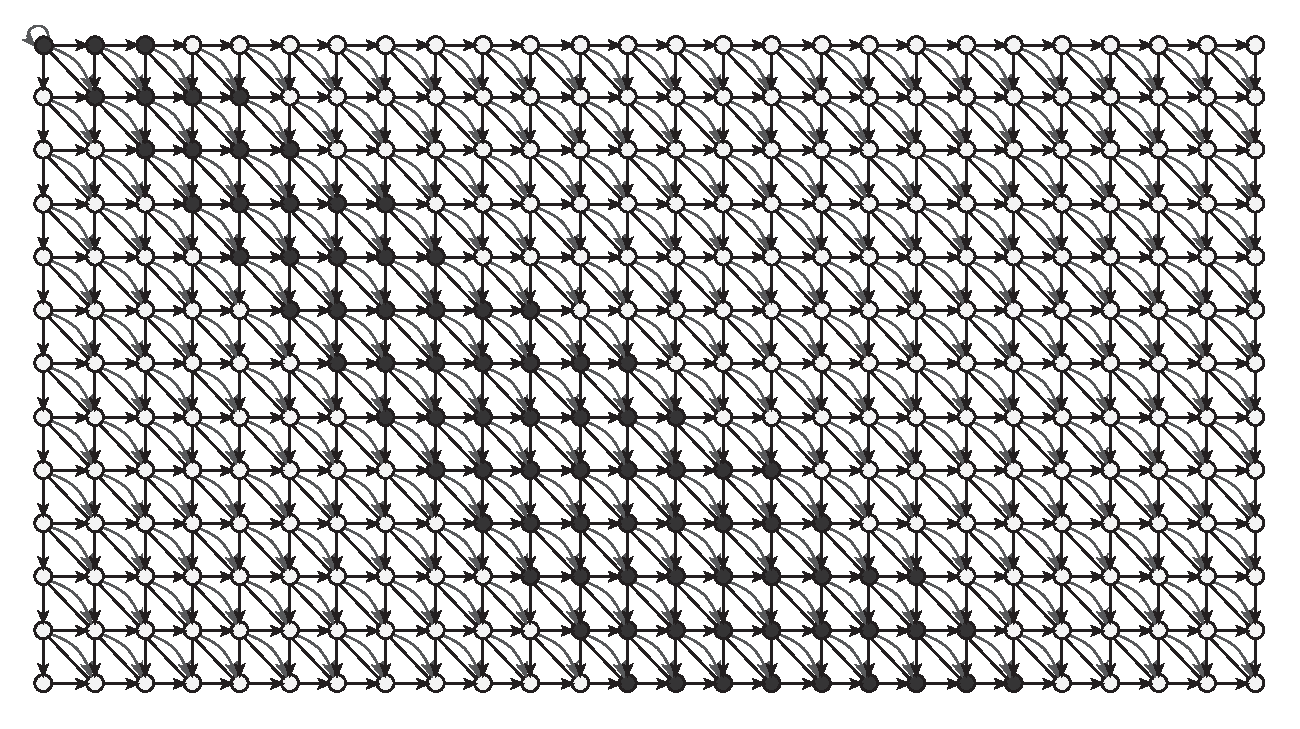
\includegraphics[scale=0.24]{sparsity_of_the_DFA.pdf}}
\caption{The Levenshtein automaton of Seeq is sparse. The sketch
represents the edit graph for a pattern of length 20 with 12
tolerated errors. The dark dots cover a region where active
states are approximately 90-95\% of the time. This region is
substantially smaller than the full edit graph and contains
221,930 different DFA states.
}\label{sparsity}
\end{figure}

It is not trivial to compute the number of states in this region
in general terms, however it can be done for the example above.
There are 221,930 states \textit{i.e.} only $0.006\%$ of the
$3.5 \cdot 10^9$ upper bound computed from the formula provided by
reviewer 2. This is of course a heuristic argument that does not
resist worst case analysis. But the upshot is that on average,
Seeq needs to store very few states of the Levenshtein automaton.

\section{Performance}

The sketch of analysis above explains all the properties of Seeq.
Because the number of states is much lower than expected, Seeq
rarely needs to use dynamic programming to compute a new state.
As an added benefit, there will be few cache misses because
most of the time, Seeq only references the same small
set of sates.

Let us give a few examples to highlight the behavior of the
algorithm. When searching the 20 nucleotide pattern
\texttt{GATGTAGCGCGATTAGCCTG}
in hg19 with up to 4 errors, Seeq ended with 5,294 states and spent
0.01\% of the time in dynamic programming. Even though
it had to scan the whole genome, the run was executed in 27 seconds,
compared to 54 seconds for Linux \texttt{wc}, which only counts the
number of characters, words and lines. On such problems where the
number of operations per character is small, the function used to read
the file makes the difference. We use GNU's \texttt{readline} because
it was faster than the alternatives in our tests.

Allowing 12 errors, which is the case of the sketch
of proof given in section \ref{sketch}, Seeq ended with 170,679 states,
close to our approximation. In this case, the running time
was 1 minute 18 seconds, of which 0.39 seconds were spent in dynamic
programming. So the difference with the previous case is either
due to cache misses or to the additional time required to process
the hits (of which there is a lot in this example), or both.

What about longer patterns with higher error tolerance?
When searching the 42 nucleotide pattern
\texttt{GATGTAGCGCGATTAGCCTGAAAATGCGAGTACGGCGCGAAT} with
up to 12 errors, Seeq ran for 2 minutes 11 seconds and ended with
3,486,701 states. About 20 seconds were spent in dynamic programming,
which shows that it is not the bottleneck.
Even with very efficient vectorization to speed up this step, the
performance of Seeq would not improve substantially. The increase
in running time is more likely due to the increased number of cache
misses.

In comparison, Myers' bitfield algorithm ran for 66 minutes
44 seconds on this problem. %Counting 17 operations per character,
%this is about 75 ns per operation, which is the right order of
%magnitude. For the bitfield algorithm to beat Seeq on the last problem,
%each operation would have to be processed in less than 2.3 ns.
We were very surprised by this result, because Myers' bitfield
algorithm has the reputation of being the fastest known alignment
algorithm. But it needs to do 17 operations per character, whereas
most of the time Seeq does just 1, and it is often a cache hit. On
the last example, Seeq performs 1 operation on 99.7\% of the
nucleotides. In summary, Myers' bitfield is not the fastest
alignment algorithm, it is the fastest alignment algorithm with
no memory footprint.

If lazy Levenshtein automata are so good, why were they not used
widely before? This is a good question. We surmise that this has
to do with the evolution of hardware. At the time they were proposed
in bioinformatics, \textit{i.e.} at the end of the 1990's, computers
typically had around 100 Mb of RAM, so they were probably considered
memory hungry and other methods filled the niche.

It is important to note that in the last case, the memory footprint
peaked at 1.5 Gb, which is approximately 430 bytes per state. The
states of the DFA proper are only an array of 5 pointers (40 bytes),
but Seeq indexes them in a ternary tree, which represents the bulk
of the memory usage. So it is true that the number of states will
become intractable for very large patterns and very high number of
tolerated errors.



\section{Concluding remarks}

We still believe that Seeq has an interesting message for the
bioinformatics community. It is certainly not the right tool for
every job, it is not intended to replace BLAST or BWA. Yet there
is a sweet spot for pattens of tens of nucleotides where we
reach good performance even for a big number of tolerated errors.

Most sequences of 20-30 nt are unique, even in large genomes,
which is why spike-ins, watermarks, adapters, barcodes and
other artificial sequences that need to be identified in sequencing
experiments will be in this range. The target application of 
Seeq is thus the Python library because it allows to easily write
parsers to identify the pattern and further process the reads as
simple Python strings.

We are aware that the information provided here would have made
the manuscript much stronger, but with a two page limit we had to
remove important parts. The difficulty was that Seeq is not novel
enough to deserve a full feature article, and it is too complex
to be described in just two pages.
We decided to present Seeq from the
perspective of the user, explain the principle and show the
performance. To be honest, we thought that there would be a
round of revisions where we could explain all this and decide
together with the reviewers how much should go in the article.
We realize now that we did not do a very good job at explaining
why Seeq is interesting. But we learned our lessons, we will do
better next time.

\section{References}

[1] https://swtch.com/~rsc/regexp/regexp1.html
\par\noindent
[2] http://blog.notdot.net/2010/07/Damn-Cool-Algorithms-Levenshtein-Automata

\end{document}
